\section{Physics-Informed Neural Networks}\label{sec:pinns}


\begin{frame}{Physics-Informed Neural Network (PINN)}
\begin{itemize}
    \item Specificity of PINNs: the loss function takes the form of a physical equation
    \item The PINN method is a meshless solution technique, finding the solutions by minimizing a loss function
    \item Ability to solve problems with very little, or noisy data.
    
\end{itemize}
    
\end{frame}



\begin{frame}{Definition of a PINN}
    \begin{enumerate}
        \item Solution $u(z)$ is approximated by a neural network parameterized by a set of parameters $\theta$
        \item For a general differential equation 
        \begin{equation*}
            \label{eq:pde-exemple}
            u_t + \mathcal{F}[u;\lambda] = 0\text{, } x\in \Omega\text{, } t \in [0, T]\text{,}
        \end{equation*} we set
        \begin{equation*}
            p \coloneqq u_t - \mathcal{F}[u;\lambda] \text{.}
        \end{equation*} This function $p$ is referred to as a \emph{physics-informed neural network}.
        \item The network learns to approximate the solution by finding the set of parameters $\theta$ that minimizes a loss function $\mathcal{L}(\theta)$
    \end{enumerate}
\end{frame}

\begin{frame}{Specific Loss Function}
    In the case of a PINN, the loss function is a sum of three components:

    \begin{itemize}
        \item The PDE residual loss 
        \item The boundary loss
        \item The data loss
    \end{itemize}

    \begin{equation*}
        \label{eq:loss-galaxy}
        \mathcal{L}(\theta) = \dfrac{1}{N_c}\sum^{N_c}_{i=1} \left\|\nabla^2 \hat{\Phi}(z_i) - 4 \pi G \rho(z_i) \right\|^2 + \dfrac{1}{N_{d}}\sum^{N_{d}}_{i=1} \left\|\hat{\Phi}(z_i) - \Phi_i \right\|^2
    \end{equation*}


\end{frame}

% \begin{frame}{Applications}
%     \begin{itemize}
%         \item Forward Problem
%         \item Inverse Problem
%     \end{itemize}
% \end{frame}
\begin{frame}{Summary}
    \begin{figure}[ht]
    \centering
    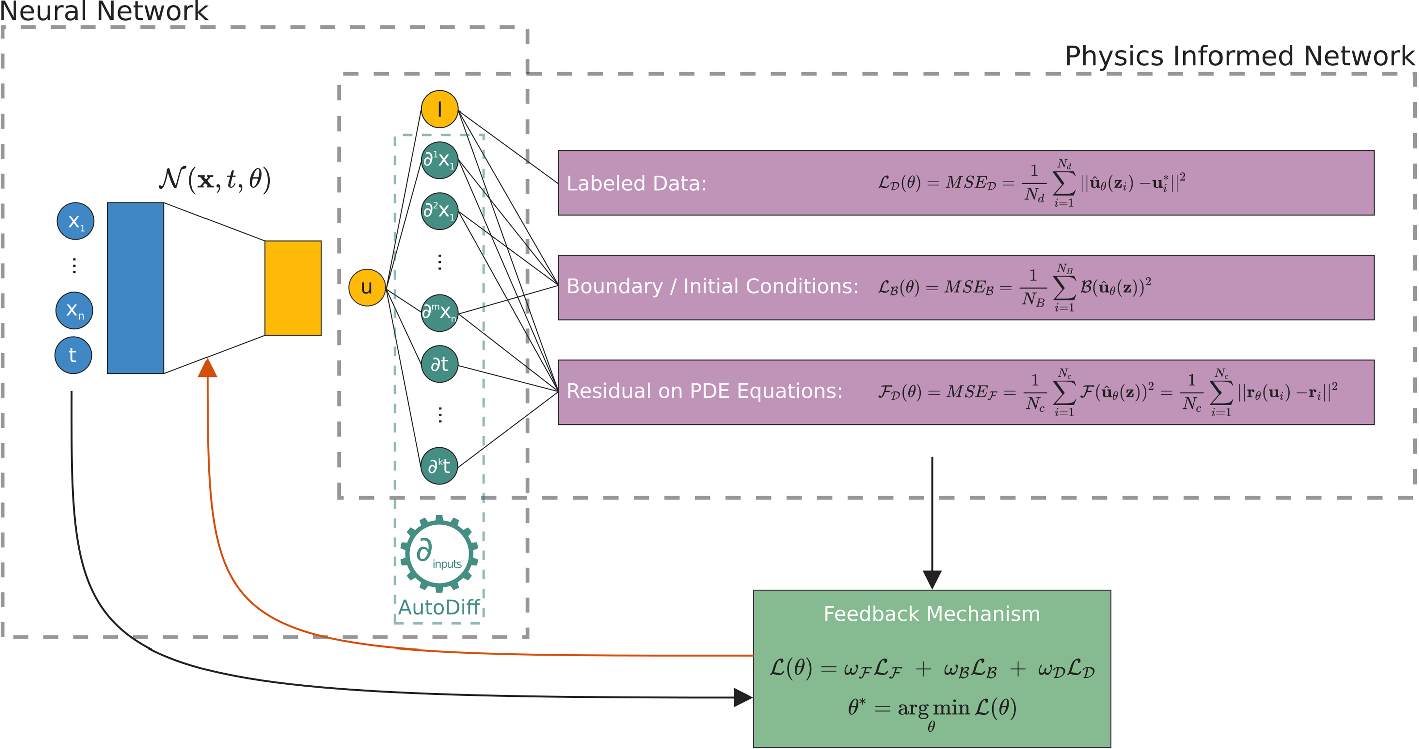
\includegraphics[scale=0.2]{imgs/training-pinn-schema.png}
    \caption{Structure and training procedure of a PINN. \textit{Illustration from~\cite{cuomo_scientific_2022}}.}
    \label{fig:loss-pinn}
\end{figure}

\end{frame}
